\section{Methodology}

This section outlines the methodological framework adopted for this study on predicting solar power generation. The approach leverages machine learning techniques, specifically LASSO Regression with and without cross-validation, and k-Nearest Neighbors (kNN) with and without hyperparameter tuning, to model the relationship between weather conditions, lagged features, and DC power output. 

\subsection{Data}

The project utilizes two datasets sourced from the "Solar Power Generation Data" repository available in Kaggle \cite{solar-kaggle}:

\begin{enumerate}
   \item \textbf{Generation Data:} This dataset encompasses records of DC power, AC power, daily yield, and total yield, all captured at 15-minute intervals across a span of 34 days.
   \item \textbf{Weather Sensor Data:} This dataset provides readings for ambient temperature, module temperature, and irradiation, also recorded at 15-minute intervals over the same 34-day period.
\end{enumerate} 

\begin{figure}[!htpb]
    \centering
    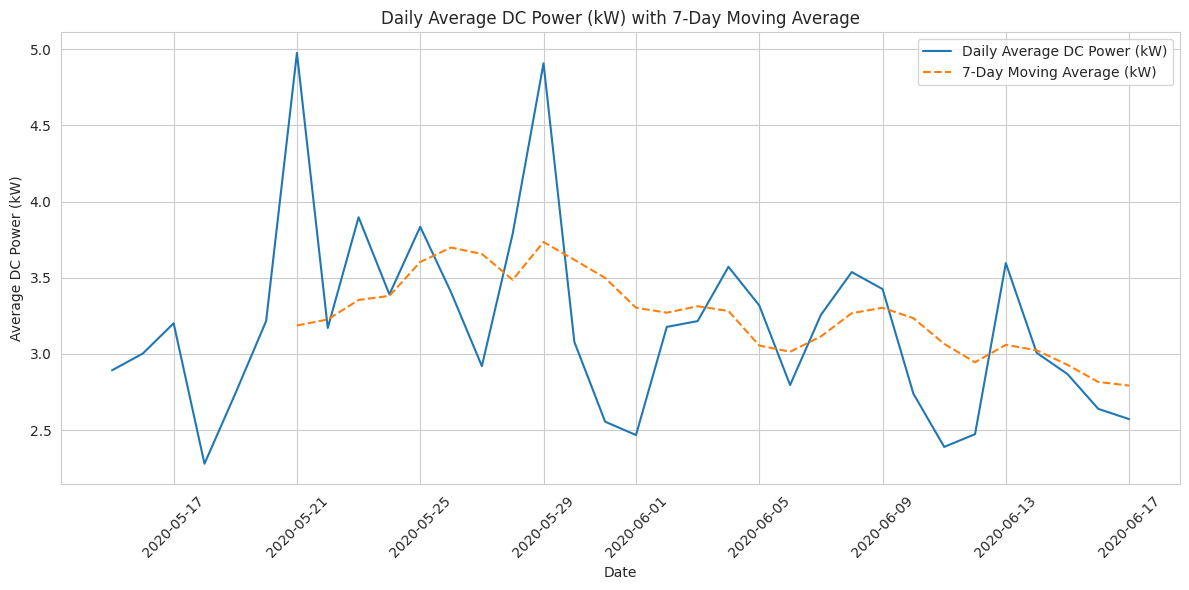
\includegraphics[width=\linewidth]{Figures/dc_by_date_f.png}
    \caption{Average DC Power by Date and 7-Day Moving Average}
    \label{fig:dc_by_date}
\end{figure}

\begin{figure}[!htpb]
    \centering
    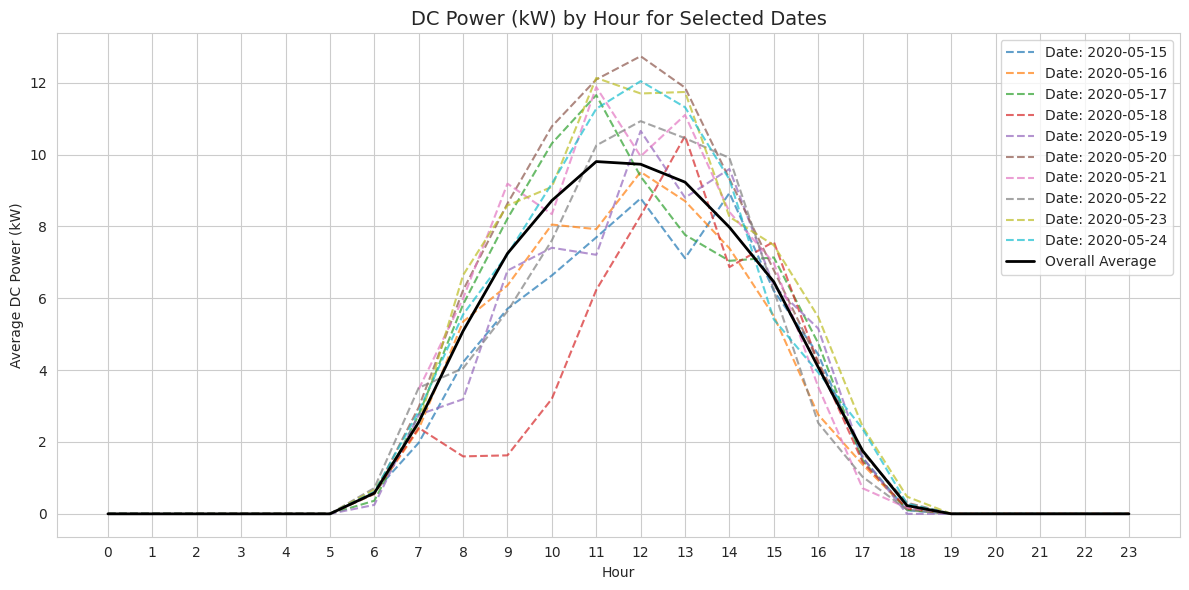
\includegraphics[width=\linewidth]{Figures/dc_by_hour_f.png}
    \caption{DC Power by Hour for a Selection of Dates and Overall Mean of the Entire Data}
    \label{fig:dc_by_hour}
\end{figure}

A brief exploratory analysis of the daily and hourly DC power generation patterns, visualized in Figure \ref{fig:dc_by_date} and Figure \ref{fig:dc_by_hour}, provide insights into the typical power output behavior and the influence of daily and hourly cycles.

\subsection{Data Preprocessing}

Prior to model training and analysis, the raw datasets underwent a series of preprocessing steps:

\begin{enumerate}
   \item \textbf{Data Loading and Resampling:} Both datasets were loaded into the Python environment, with the date-time columns being converted into a consistent and analysis-friendly format. The initial 15-minute frequency of data collection was resampled into two different datasets with both daily and hourly aggregations. This provided flexibility in exploring models sensitive to different temporal resolutions.
   \item \textbf{Merging Datasets:} The generation and weather data were merged into a unified dataset based on their corresponding date-time stamps. This ensured that weather features and power generation values were properly aligned for each observation.
   \item \textbf{Feature Engineering:} Lagged features, representing past values of DC power and weather variables, were generated. These lagged features aimed to capture potential time-dependent patterns and enhance the predictive power of the models.
   \item \textbf{Imputation:} The KNN Imputer was employed to address any remaining missing values in the dataset. This method leverages the values of neighboring data points to estimate and fill in missing entries, preserving data integrity for model training.
\end{enumerate} 

It is important to note that data normalization was skipped, despite it usually being a crucial step in machine learning pipelines, to preserve the original scale of the data and provide a clearer sense of the models' performance metrics.

\subsection{Model}

This study explored both linear and non-linear modeling approaches, with variations in hyperparameter settings, to comprehensively evaluate their effectiveness in predicting DC power generation:

\begin{enumerate}
   \item \textbf{LASSO Regression:} A linear regression technique that incorporates L1 regularization, adding a penalty to model complexity and shrinking coefficients of less important features. This model was implemented with a default regularization parameter.
   \item \textbf{LassoCV (LASSO Regression with Cross-Validation):} Extends LASSO regression by using cross-validation to find the optimal regularization parameter (\(\lambda\)).  LassoCV tested a range of  \(\lambda\) values from 0.001 to 1 to prevent overfitting and select relevant features. Time series cross-validation (TimeSeriesSplit), implementation as seen in Figure \ref{fig:time_series_split} was specifically employed to respect the temporal order of the data during model evaluation.
   \item \textbf{kNN (k-Nearest Neighbors):} A non-parametric method that predicts an output based on the values of its \emph{k} nearest neighbors in the feature space. This model was implemented using hyperparameter tuning for an automated selection of the best \emph{k} neighbors. The model explored \emph{k} values from 3 to 6 to minimize prediction error. 
   \item \textbf{kNN with Cross-Validation:} Improves upon the basic kNN by using cross-validation on top of hyperparameter tuning to determine the optimal number of neighbors (\emph{k}). Similar to LassoCV, time series cross-validation was used to maintain temporal consistency during model assessment. 
\end{enumerate} 

\begin{figure}[!htpb]
    \centering
    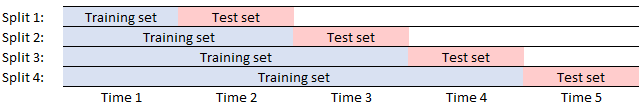
\includegraphics[width=\linewidth]{Figures/time_series_split.png}
    \caption{Expanding Window in scikit-learn's TimeSeriesSplit}
    \label{fig:time_series_split}
\end{figure}

All models were trained using an 80\% split of the data and tested on the remaining 20\%, with a temporally consistent division without shuffling to preserve the continuity of the time series and prevent data leakage.

\subsection{Experiments}

Here, and in the proceeding sections we abbreviate several terms: $D$ for DC power, $A$ for ambient temperature, $M$ for module temperature, and $I$ for irradiation. To evaluate the performance of LASSO and kNN under various scenarios, the following experiments were designed:

\begin{enumerate}

   \item \textbf{Univariate One-day-ahead Prediction with 1 Lag:} This experiment focused on predicting the current day's average DC power solely based on the previous day's average DC power.

\begin{tikzpicture}[
  node distance=.1cm and 1.2cm,
  feature/.style={draw=none},
  target/.style={draw=none}
]

% Matrix with reduced column separation
\matrix (matrix1) [matrix of nodes, column sep=5pt] {
  $\bar{D_0}$ \\ 
  $\bar{D_1}$ \\ 
  \vdots \\
  $\bar{D_{25}}$ \\
  $\bar{D_{26}}$ \\
  $\bar{D_{27}}$  \\
  \vdots \\
  $\bar{D_{32}}$ \\ 
};

% Target column (D) - referencing matrix nodes
\node[target,right=of matrix1-1-1] (D1t) {$\bar{D_1}$};
\node[target,right=of matrix1-2-1] (D2t) {$\bar{D_2}$};
\node[target,below=.001cm of D2t] (dots2) {$\vdots$};
\node[target,right=of matrix1-4-1] (D26t) {$\bar{D_{26}}$};
\node[target,right=of matrix1-5-1] (D27t) {$\bar{D_{27}}$};
\node[target,right=of matrix1-6-1] (D28t) {$\bar{D_{28}}$};
\node[target,below=.001cm of D28t] (dots4) {$\vdots$};
\node[target,right=of matrix1-8-1] (D33t) {$\bar{D_{33}}$};

% Arrows - referencing matrix nodes
\draw[->] (matrix1-1-1) -- node[above,midway,red] {Day 1} (D1t);
\draw[->] (matrix1-2-1) -- node[above,midway,red] {Day 2} (D2t);
\draw[->] (matrix1-4-1) -- node[above,midway,red] {Day 26} (D26t);
\draw[->] (matrix1-5-1) -- node[above,midway,red] {Day 27} (D27t);
\draw[->] (matrix1-6-1) -- node[above,midway,red] {Day 28} (D28t);
\draw[->] (matrix1-8-1) -- node[above,midway,red] {Day 33} (D33t);

\end{tikzpicture}

   \item \textbf{Multivariate (Multiple Features) One-day-ahead Prediction with 1 Lag:} This experiment expanded upon the previous one by incorporating additional lagged features, including daily average ambient temperature, module temperature, and irradiation. The goal was to assess whether the inclusion of these extra features improved predictive accuracy.

\begin{tikzpicture}[
  node distance=.1cm and 1.2cm,
  feature/.style={draw=none},
  target/.style={draw=none}
]

% Matrix with reduced column separation
\matrix (matrix1) [matrix of nodes, column sep=5pt] {
  $\bar{D_0}$ & $\bar{I_0}$ & $\bar{A_0}$ & $\bar{M_0}$ \\ 
  $\bar{D_1}$ & $\bar{I_1}$ & $\bar{A_1}$ & $\bar{M_1}$ \\ 
  \vdots & \vdots & \vdots & \vdots \\
  $\bar{D_{25}}$ & $\bar{I_{25}}$ & $\bar{A_{25}}$ & $\bar{M_{25}}$ \\
  $\bar{D_{26}}$ & $\bar{I_{26}}$ & $\bar{A_{26}}$ & $\bar{M_{26}}$ \\
  $\bar{D_{27}}$ & $\bar{I_{27}}$ & $\bar{A_{27}}$ & $\bar{M_{27}}$ \\
  \vdots & \vdots & \vdots & \vdots \\
  $\bar{D_{32}}$ & $\bar{I_{32}}$ & $\bar{A_{32}}$ & $\bar{M_{32}}$ \\ 
};

% Target column (D) - referencing matrix nodes
\node[target,right=of matrix1-1-4] (D1t) {$\bar{D_1}$};
\node[target,right=of matrix1-2-4] (D2t) {$\bar{D_2}$};
\node[target,below=.001cm of D2t] (dots2) {$\vdots$};
\node[target,right=of matrix1-4-4] (D26t) {$\bar{D_{26}}$};
\node[target,right=of matrix1-5-4] (D27t) {$\bar{D_{27}}$};
\node[target,right=of matrix1-6-4] (D28t) {$\bar{D_{28}}$};
\node[target,below=.001cm of D28t] (dots4) {$\vdots$};
\node[target,right=of matrix1-8-4] (D33t) {$\bar{D_{33}}$};

% Arrows - referencing matrix nodes
\draw[->] (matrix1-1-4) -- node[above,midway,red] {Day 1} (D1t);
\draw[->] (matrix1-2-4) -- node[above,midway,red] {Day 2} (D2t);
\draw[->] (matrix1-4-4) -- node[above,midway,red] {Day 26} (D26t);
\draw[->] (matrix1-5-4) -- node[above,midway,red] {Day 27} (D27t);
\draw[->] (matrix1-6-4) -- node[above,midway,red] {Day 28} (D28t);
\draw[->] (matrix1-8-4) -- node[above,midway,red] {Day 33} (D33t);

\end{tikzpicture}

   \item \textbf{Multivariate (Hourly Train Data as Features) One-day-ahead Prediction with 1 Lag:} Recognizing the potential value of higher temporal granularity, this experiment used the previous day hourly weather data and lagged features to predict current day average DC power. Various combinations of features were explored through feature selection.

\begin{tikzpicture}[
  node distance=.1cm and 1.2cm,
  feature/.style={draw=none},
  target/.style={draw=none}
]

% Matrix with reduced column separation and repeated elements
\matrix (matrix1) [matrix of nodes, column sep=5pt, nodes={align=center}] {
  $D^1_0$ & \dots & $D^{24}_0$  & \dots & $I^1_0$ & \dots & $I^{24}_0$ \\[-3pt]
  $D^1_1$ & \dots & $D^{24}_1$  & \dots & $I^1_1$ & \dots & $I^{24}_1$ \\[-3pt] 
  \vdots &  & \vdots & & \vdots &  & \vdots \\
  $D^1_{25}$ & \dots & $D^{24}_{25}$  & \dots & $I^1_{25}$ & \dots & $I^{24}_{25}$ \\[-3pt] 
  $D^1_{26}$ & \dots & $D^{24}_{26}$  & \dots & $I^1_{26}$ & \dots & $I^{24}_{26}$ \\[-3pt]
  $D^1_{27}$ & \dots & $D^{24}_{27}$  & \dots & $I^1_{27}$ & \dots & $I^{24}_{27}$ \\[-3pt]
  \vdots &  & \vdots & & \vdots &  & \vdots \\
  $D^1_{32}$ & \dots & $D^{24}_{32}$  & \dots & $I^1_{32}$ & \dots & $I^{24}_{32}$ \\ 
};

% Target column (D) - referencing matrix nodes
\node[target,right=of matrix1-1-7] (D1t) {$\bar{D_1}$};
\node[target,right=of matrix1-2-7] (D2t) {$\bar{D_2}$};
\node[target,below=-0.1cm of D2t] (dots2) {$\vdots$};
\node[target,right=of matrix1-4-7] (D26t) {$\bar{D_{26}}$};
\node[target,right=of matrix1-5-7] (D27t) {$\bar{D_{27}}$};
\node[target,right=of matrix1-6-7] (D28t) {$\bar{D_{28}}$};
\node[target,below=-0.1cm of D28t] (dots4) {$\vdots$};
\node[target,right=of matrix1-8-7] (D33t) {$\bar{D_{33}}$};

% Arrows - referencing matrix nodes
\draw[->] (matrix1-1-7) -- node[above,midway,red] {Day 1} (D1t);
\draw[->] (matrix1-2-7) -- node[above,midway,red] {Day 2} (D2t);
\draw[->] (matrix1-4-7) -- node[above,midway,red] {Day 26} (D26t);
\draw[->] (matrix1-5-7) -- node[above,midway,red] {Day 27} (D27t);
\draw[->] (matrix1-6-7) -- node[above,midway,red] {Day 28} (D28t);
\draw[->] (matrix1-8-7) -- node[above,midway,red] {Day 33} (D33t);

\end{tikzpicture}

\end{enumerate} 

\subsection{Evaluation}

Model performance was rigorously evaluated using the Root Mean Squared Error (RMSE) metric. RMSE quantifies the average magnitude of prediction errors, providing a measure of how well the model's predictions align with the actual DC power values. Lower RMSE values indicate better predictive accuracy.

$RMSE: \sqrt{\frac{1}{6}\sum_{i=1}^{6} \left[ (y_{test})_i - Model.Predict(x_{test})_i \right]^2}$

A comparative analysis of RMSE scores across all experiments helped determine the most effective modeling approach for this specific problem. The analysis considered factors such as feature set selection, temporal resolution of the data, and the influence of hyperparameter tuning on each model's predictive accuracy.